\documentclass[11pt,a4paper]{report}

\PassOptionsToPackage{dvipsnames}{xcolor}

\usepackage{url}
\usepackage[utf8]{inputenc}
\usepackage{graphicx}
\usepackage[all]{xy}
\usepackage{amsmath}
\usepackage{amsthm}
\usepackage[colorinlistoftodos,prependcaption,textsize=tiny]{todonotes}
\usepackage{array}
\usepackage{xcolor}
\usepackage{listings}
\usepackage[a4paper]{geometry}
\usepackage{float}
\usepackage{hyperref}
\usepackage{tikz}
\usepackage{xargs}

%
\newcommandx{\unsure}[2][1=]{\todo[linecolor=red,backgroundcolor=red!25,bordercolor=red,#1]{#2}}
\newcommandx{\change}[2][1=]{\todo[linecolor=blue,backgroundcolor=blue!25,bordercolor=blue,#1]{#2}}
\newcommandx{\info}[2][1=]{\todo[linecolor=OliveGreen,backgroundcolor=OliveGreen!25,bordercolor=OliveGreen,#1]{#2}}
\newcommandx{\improvement}[2][1=]{\todo[linecolor=Plum,backgroundcolor=Plum!25,bordercolor=Plum,#1]{#2}}
\newcommandx{\thiswillnotshow}[2][1=]{\todo[disable,#1]{#2}}
%

\makeatletter %otherwise geometry resets everything
\Gm@restore@org
\makeatother

\setlength{\itemsep}{0cm}
\setlength{\voffset}{0cm}
\setlength{\headheight}{0cm}
\setlength{\topmargin}{0cm}
\setlength{\extrarowheight}{3pt} %for superscripts in tabular
\setlength{\arraycolsep}{4pt}
\lstset{basicstyle = \footnotesize, breaklines = true}

\graphicspath{{imgs/}}

\begin{document}
\begin{titlepage}
\begin{center}
\textsc{\LARGE Master thesis\\Data Science}[1.5cm]
\includegraphics[height=100pt]{logo}

\vspace{0.4cm}
\textsc{\Large Radboud University}[1cm]
\hrule
\vspace{0.4cm}
\textbf{\huge Using fast inpainting transformers for anomaly detection\\[0.3cm]
\LARGE  
}[0.4cm]
\hrule
\vspace{2cm}
\begin{minipage}[t]{0.45\textwidth}
\begin{flushleft} \large
\textit{Author:}\\
Sébastiaan Versteeg, BSc\\
\texttt{hello@sebastiaan.app}
\end{flushleft}
\end{minipage}
\begin{minipage}[t]{0.45\textwidth}
\begin{flushright} \large
\textit{First supervisor:}\\
Prof.dr. E Marchiori\\
\texttt{elenam@cs.ru.nl}\\[1.3cm]
\textit{Second assessor:}\\
Firstname Lastname\\
\texttt{email@example.com}
\end{flushright}
\end{minipage}
\vfill
{\large \today}
\end{center}
\end{titlepage}

\begin{abstract}
The detection and segmentation of irregularities in images is an anomaly detection problem in computer vision. An approach that is used commonly uses autoencoders trained on good images to fully reconstruct anomalous images. These reconstructions can then be used to perform detection and segmentation by mathematically comparing the original input and the reconstruction. Other solutions introduce patch inpainting as a solution for anomaly detection. One approach uses an attention-based transformer model that achieves promising results. Transformers are generally slower models and thus faster versions have been proposed. We therefore combine the inpainting solution with two types of transformers and see that a linear attention approach performs slightly better than full attention when doing detection and segmentation on the MVTec AD dataset.
\end{abstract}

\renewcommand{\abstractname}{Acknowledgements}
\begin{abstract}
 Thanks Mum!
\end{abstract}
\tableofcontents

\chapter{Introduction}\label{ch:introduction}

The detection of deviations in data is an important topic in multiple fields. Examples of these include medical imaging \cite{han_madgan_2021}, surveillance \cite{shashikar_traffic_2017} and manufacturing \cite{susto_anomaly_2017}. These types of anomaly detection aim to find irregularities in different types of images.

\improvement{Elaborate more on why anomaly detection is useful exactly}

Notably self-supervised anomaly detection is an approach that has been explored recently \cite{li_cutpaste_2021, ali_self-supervised_2020}. This type of machine learning means that we use unlabeled data to train our models. We can use examples of normal situations to be able to reconstruct full images where the anomaly has been removed. This allows us to compare a source image to a reconstruction and find any anomalies. This method using image inpainting has been implemented using various methods like generative adversarial networks (GANs) \cite{yeh_semantic_2017} and transformers \cite{pirnay_inpainting_2021}.


Transformers \cite{vaswani_attention_2017} are a type of model that is based on self-attention. This attention processes a lot of context, which makes the training of these types of models slow. Therefore different implementations have been explored, like linear transformers \cite{katharopoulos_transformers_2020}, fastformers \cite{wu_fastformer_2021} and linformers \cite{wang_linformer_2020}.

Since the linear transformers seem to have some performance improvement over the vanilla transformers we see an opportunity to use these newer type of transformer in the context of image inpainting for anomaly detection. We propose to use the method used by Pirnay et al. \cite{pirnay_inpainting_2021} but replace the used transformer by the linear transformer introduced by Katharopoulos et al. \cite{katharopoulos_transformers_2020}. Thus we ask:

\textit{What is the effect on the performance and efficiency of using linear transformers in an inpainting context for anomaly detection when compared to regular transformers?}

To be able to compare the different models we ask a few subquestions:
\todo{Need to rephrase and change questions if necessary based on data}
\begin{itemize}
    % inpainting/anomaly detection
    \item What are easy and hard images for the model?
    \item Are there correlations between hard and easy cases?
    % performance/efficiency
    \item How does the training time compare between types of images?
    \item How does the training time compare between different types of models?
    % linear vs regular
    \item How do our results compare to previous work?
\end{itemize}

We will answer this by doing an in-depth analysis of using linear transformers compared to regular transformers.

\improvement{Insert section about thesis structure in general}
\chapter{Preliminaries}\label{ch:preliminaries}

\section{Types of machine learning}
\label{sec:prelim:types-of-machine-learning}

There are different approaches to machine learning. In this section we will introduce a few of these approaches to give context for our research.


\subsection{Supervised learning}

Supervised learning \cite{mohri_foundations_2012} is a type of machine learning approach that always uses a labeled dataset to train a model. This means that for each point in the dataset we already know what class or rank it belongs to. It is the common type of learning used with problems that require classification, regression or ranking. The known samples are used to train a model and to make predictions for data points that the model has not yet seen.

An example would be making predictions about images of animals. Each image would be labeled with the type of animal that is in the picture. Use that data we would be learning our models to be able to predict the type of animal in pictures that the model has never seen before.

\subsection{Unsupervised learning}

This subset of machine learning focuses on training models with unlabeled data. Examples of problems that use this type of learning are clustering and dimensionality reduction. For unsupervised methods it is hard to measure the performance quantitatively because there are no labels to compare the results to.

An example of this type would be clustering people by known information like age, education or income. The goal here is to split the dataset based on information that is similar between the points. So only the points from the dataset are used to create a result, there is no previous knowledge about the data that can be used.

\subsection{Self-supervised learning}

The type of machine learning that we use in this thesis is a form of self-supervised learning \cite{doersch_multi-task_2017}. This means that we generate our own labels from a dataset without any manual work required. This is possible by removing or modifying part of the input data and then learn a model to recover the original data. We can measure the performance based on the difference between the original data and the result. This type of learning can be seen as a combination of unsupervised and supervised learning.

An example is a model that tries to predict words in a certain context. We have a sentence: 'The most popular food from France is the croissant'. We can then leave out the word 'croissant' and train a model to predict the word based on the words surrounding it.

\section{Transformers}
\label{sec:prelim:transformers}

The type of model used in our research is a transformer. In this section we will introduce the attention mechanism, explain how this is used in transformers and how this is affecting the kind of transformer we are using.

\subsection{Vanilla transformers}
\label{sec:prelim:transformers:vanilla}

In 2017 Vaswani et al.\cite{vaswani_attention_2017} introduced the transformer model. A type of sequence to sequence model that uses an attention mechanism as the main building block. This allowed them to increase parallelisation and reach a new state of the art in the context of language translations.

\subsubsection{Architecture}

The transformer model uses the same encoder-decoder structure used in the models it was compared to in the original paper \cite{bahdanau_neural_2016, cho_learning_2014}. This means that the model consists of two parts: an encoder and a decoder.

The encoder takes an input representation $(x_1,...x_n)$ and transforms this to an intermediary representation $(z_1,...z_n)$. This intermediary representation is then used as input for the decoder to create an output $(y_1,...,y_n)$.

\begin{figure}[ht]
\centering
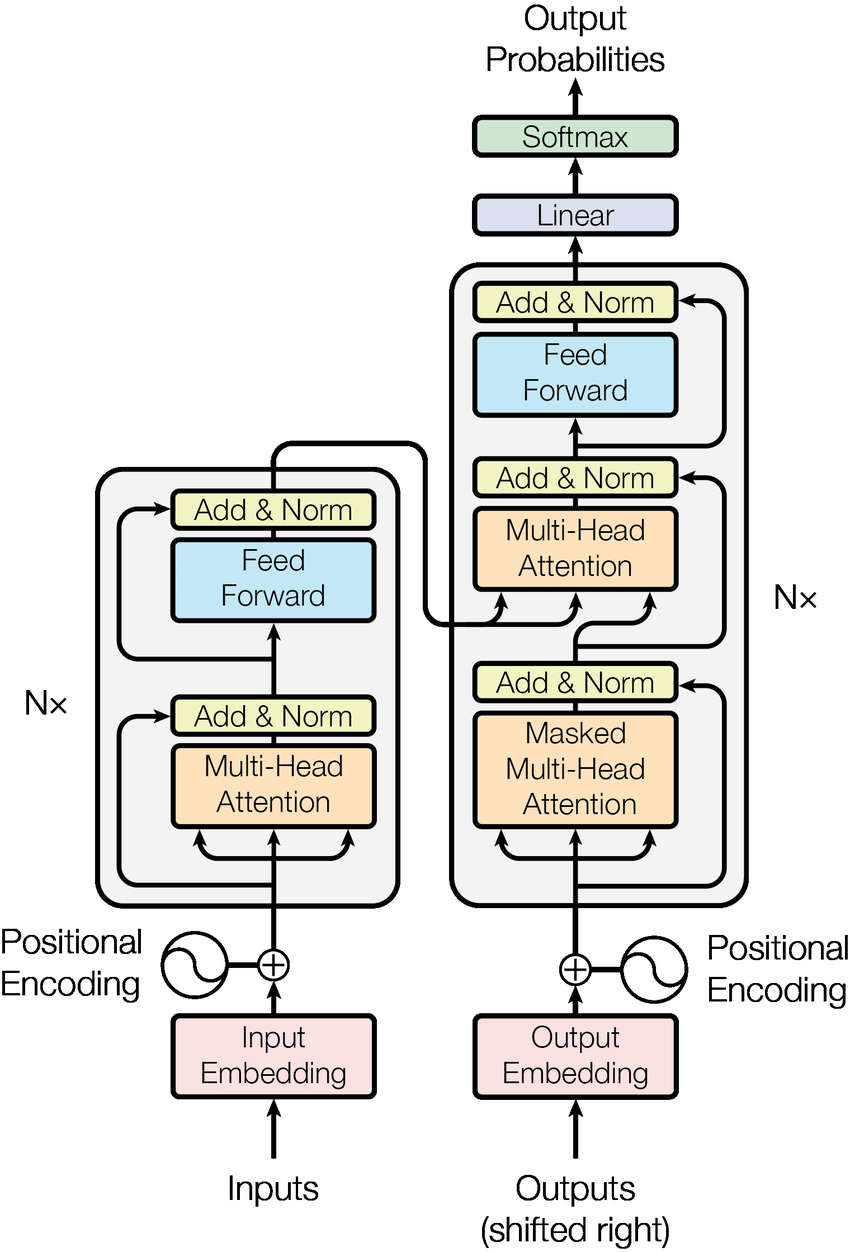
\includegraphics[width=0.5\textwidth]{transformer.png}
\caption{The original transformer architecture from \cite{vaswani_attention_2017}}
\label{fig:prelim:transformer-architecture}
\end{figure}


\paragraph{Attention}

The attention mechanism, which takes query, keys and values vector as input, outputs a vector containing a weighted sum of the values. Each of the output values uses a weight that is calculated using a compatibility  function of the query and the key in each position.

The attention mechanism \cite{vaswani_attention_2017} is called 'Scaled Dot-Product Attention' or softmax attention and calculates attention using matrices that consist of multiple vectors packed together. These matrices are $Q$ (queries), $K$ (keys) and $V$ (values) of dimension $S \times d_k$, $d_k \times S$ and $S \times d_v$ where $S$ is the sequence length of vectors:
\begin{align}
\label{eq:prelim:softmax-attention}
&Attention(Q, K, V) = softmax(\frac{QK^T} {\sqrt{d_k}})V
\end{align}

To be able to apply the attention to more than one representation space we use multi-headed attention. This uses $h$ parallel layers that all attend to a smaller part of the full dimension. In the case of the original papers $h = 8$ and the dimension of each attention head becomes $d_k = d_v = D / h = 64$ when $D = 512$. This makes the multi-headed attention similar to single-head attention with the full dimension when we look at the computational cost.

To combine the results of the attention heads we learn linear projections ($W_i^Q$, $W_i^K$, $W_i^V$) that we project all queries, keys and values to. All the separate outputs of the different attention heads are concatenated and projected into the correct dimension , which gives us the final output.

\begin{align}
&MultiHead(Q, K, V) = Concat(head_1, ..., head_h)W^O\\
& where\ head_i = Attention(QW_i^Q, KW_i^K, VW_i^V)
\end{align}


\paragraph{Encoder}
The encoder part in the architecture is a stack of $N$ layers. All the layers are the same and consist of two sublayers: the multi-head self-attention and a fully-connected feed-forward network (FFN). After both sublayers we apply layer normalisation\cite{ba_layer_2016} and add residual connections\cite{he_deep_2015} around the sublayers. This means that the output of a layer in the encoder is calculated as follows: 
\begin{align}
\label{par:prelim:transformer-encoder}
&selfAtt = LayerNorm(input + MultiHead(input_q, input_k, input_v))\\
&enc = LayerNorm(selfAtt + FFN(selfAtt))
\end{align}

where $input_q = input_k = input_v$ are the input of the encoder layer. These arguments are the same, since we are applying self-attention here.


\paragraph{Decoder}
Similar to the encoder the decoder is a stack of $N$ layers. Compared to the encoder it adds a third sublayer that applies multi-head cross attention to the output from the encoder layers and the first sublayer of the decoder. In the first self-attention sublayer we mask out earlier positions in the output sequence to stop predictions for a certain position $i$ to depend on the outputs at the positions before position $i$. The residual connections and layer normalisation on each sublayer is identical to the architecture of the encoder. This results in the following calculations for each decoder layer: 
\begin{align}
&selfAtt = LayerNorm(input + MaskedSelfAtt(input_q, input_k, input_v))\\
&crossAtt = LayerNorm(selfAtt + CrossAtt(selfAtt_q, enc_k, enc_v))\\
&dec = LayerNorm(crossAtt + FFN(crossAtt))
\end{align}

where $MaskedSelfAtt$ is the function that applies the masking before $MultiHead$, $input_q = input_k = input_v$ are the input of the decoder layer and $enc_k$ and $enc_v$ the keys and values of the encoder layers. $selfAtt_q$ are the queries from the first attention function.

The final layers consist of a linear fully connected neural network and a softmax layer. This allows us to have a higher number of possible outputs than the size of the input and output embeddings since it projects the output of the decoder part into a probability vector.

\subsection{Vision transformers}
\label{sec:prelim:transformers:vision}

As mentioned in the previous section transformers were originally meant for text problems. The success of the transformer in that context is what made Dosovitskiy et al. \cite{dosovitskiy_image_2021} start exploring the usage of the attention-based model for computer vision tasks as well.

Their approach tries to use the original transformer implementation as much as possible. This means that they had to introduce an intermediate step to be able to use the images as input for the model.

The original model is designed to receive a 1 dimensional input of token embeddings. The input images for the vision transformers are 2 dimensional and each image has the shape $x \in \mathbb{R}^{H \times W \times C}$ where $H$ and $W$ are the height and width of the image respectively and $C$ is the number of channels. To be able to use the images as input they split the image in square patches with the resolution $(P, P)$. This results in $N = HW/P^2$ patches $x_p \in \mathbb{R}^{N \times (P^2 \; \cdot \; C)}$.

To obtain the patch embeddings they first flatten the patches and then train a linear projection  mapping them to a single dimension. To this sequence of patch embeddings they prepend a learnable embedding. Then to allow for the preservation the positions of the patches, they add positional embeddings to the patch embeddings.

\subsection{Linear transformers}
\label{sec:prelim:transformers:linear}

Since transformers use attention to process so many parts of the images the model has a high memory and time complexity. One of the proposed solutions to reduce the complexity of the models is made by Katharopoulos et al. \cite{katharopoulos_transformers_2020}. They introduce the linear transformer that according to their results can reach similar performance when compared to vanilla transformers with the benefit of being faster. 

To see the advantage of their attention function we first need to understand what the bottleneck is in regular transformers. For this we look at equation \ref{eq:prelim:softmax-attention} again:

\begin{align}
&Attention(Q, K, V) = softmax(\frac{QK^T} {\sqrt{d_k}})V
\tag{\ref{eq:prelim:softmax-attention} revisited}
\end{align}

Here we apply the softmax function row-wise to $\frac{QK^T} {\sqrt{d_k}}$. This means that the complexity of the multiplication of the three matrices $Q$, $K^T$ and $V$ becomes $O(S^2 d_k)$.

The approach by Katharopoulus et al. starts by rewriting the attention calculation in equation \ref{eq:prelim:softmax-attention} into a generalised equation for any similarity function $sim(Q, K)$.

\begin{align}
&Attention(Q, K, V) = V'
\end{align}

Given that $V_i$ returns the i-th row of $V'$ as a vector:

\begin{align}
&V'_i =\frac{\sum_{j-1} ^{N} sim(Q_i, K_j) V_j}{\sum_{j-1} ^{N} sim(Q_i, K_j)}
\label{eq:prelim:general-attention}
\end{align}

This equation is equivalent to equation \ref{eq:prelim:softmax-attention} when we say $sim(q, k) = exp(\frac{q^Tk}{\sqrt{D}})$.

\\We need to set a constraint on $sim(q, k)$ for this equation to be able to define an attention function. And that is that it has to be non-negative.\\

Now given some kernel with a feature representation $\phi(x)$ we can rewrite equation \ref{eq:prelim:general-attention} as follows:

\begin{align}
    &V'_i = \frac{\sum_{j=1}^{N} \phi(Q_i)^T\phi(K_j)V_j}{\sum_{j=1}^{N} \phi(Q_i)^T\phi(K_j)}
    \label{eq:prelim:lin-att-1}
\end{align}

This is possible by using the kernel trick\footnote{https://en.wikipedia.org/wiki/Kernel_method#Mathematics:_the_kernel_trick}. We can avoid learning a non-linear function using this trick. It allows us to rewrite our similarity function as follows:

\begin{align}
sim(q, k) = \phi(q)^T\phi(k)
\end{align}

We can then simplify equation \ref{eq:prelim:lin-att-1} using the associative property of matrix multiplication to:

\begin{align}
    &V'_i = \frac{\phi(Q_i)^T\sum_{j=1}^{N} \phi(K_j)V_j^T}{\phi(Q_i)^T\sum_{j=1}^{N} \phi(K_j)}
\end{align}

In \cite{katharopoulos_transformers_2020} they note that the feature function $\phi(x)$ that corresponds to the exponential kernel $exp$ is infinite dimensional. This makes it infeasible to linearise softmax attention itself. Therefore they choose the following feature map:

\begin{align}
    \phi(x) = elu(x) + 1
\end{align}

with $elu(x)$ being the exponential linear unit activation function \cite{clevert_fast_2015}:

\begin{align}
    elu(x) =     \begin{cases}     \mbox{$x$} & \mbox{if } x > 0\\     \mbox{$\alpha (e^x-1)$} & \mbox{if } x < 0     \end{cases}
\end{align}

where $\alpha = 1.0$. This results in a complexity of $O(S d_k)$ which is no longer quadratic when compared to softmax attention.

\section{Image inpainting}
\label{sec:prelim:image-inpainting}

To be able to detect anomalies without labelling a large dataset we are using a semi-supervised method using image inpainting.

Inpainting is the process of filling in missing, damaged or censored parts in paintings or images. It can also be used for object removal or image manipulation.
Applying the technique on digital images can be done using different approaches.

\begin{figure}[ht!]
\centering
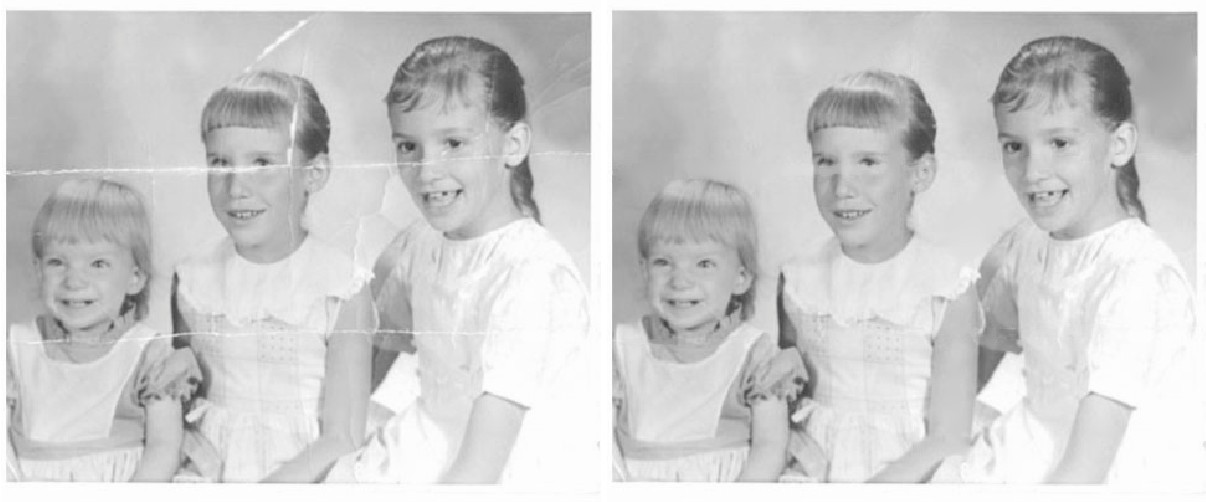
\includegraphics[width=\textwidth]{imgs/inpainting-example.jpeg}
\caption{An example of image restoration using inpainting from Bertalmio et al. \cite{bertalmio_image_2000}}
\label{fig:prelim:inpainting-example}
\end{figure}

In figure \ref{fig:prelim:inpainting-example} we see a photo that is restored by using a context based inpainting method.

Our transformer-based approach, which is modeled after the Inpainting Transformer (InTra) from Pirnay et al. \cite{pirnay_inpainting_2021} learns to paint regions that are removed from the original images. This allows the models to fully reconstruct an image based on the surrounding patches. This approach is discussed more extensively in section \ref{sec:experimental-setup:model}.

\section{Anomaly detection}
\label{sec:prelim:anomaly-detection}

Anomaly detection is the detection of outliers, points that have extreme values compared to the rest, in a dataset.
This kind of detection can be useful in different environments. Examples are intrusion detection in security and fault detection in industrial systems.

\begin{figure}[H]
\centering
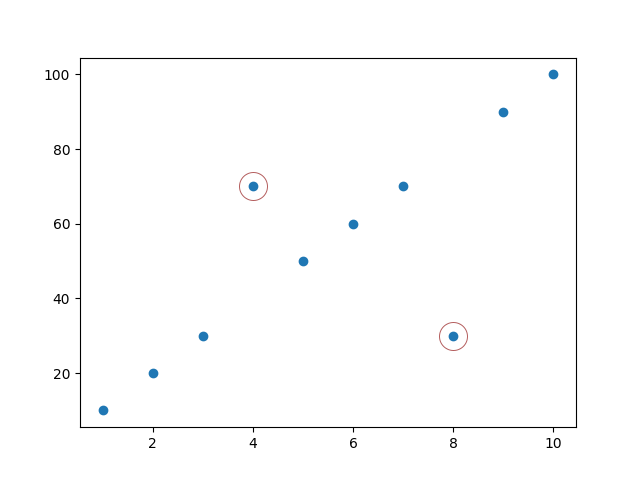
\includegraphics[]{imgs/outliers-example.png}
\caption{An example of outliers in a scatter plot}
\label{fig:prelim:outliers-example}
\end{figure}

In our case we are looking at anomalies in manufacturing. We want to find defects in images of objects and textures.

\section{Image similarity}
\label{sec:prelim:image-similarity}

To allow us to compare inpainted images to original samples from a dataset we want to use objective measures that try to approach a human visual system. For our research we use two measures specifically: Gradient Magnitude Similarity \cite{xue_gradient_2014, zhang_gradient_2017} and Structured Similarity Index \cite{wang_image_2004}.

\subsection{Structured Similarity Index}

This metric uses three features from an image to be able to make a comparison: luminance, contrast and structure. These features are taken from two images $r$ and $d$.

The luminance is an estimation of the mean intensity:

\begin{align}
    \mu_x = \frac{1}{N}\sum_{i=1}^{N}{x_i}
\end{align}

Using $\mu_r$ and $\mu_d$ we can now make a comparison function $l(r, d)$.

\begin{align}
    l(r, d) = \frac{ 2\mu_x\mu_y + C_1 }{ \mu_x^2 + \mu_y^2 + C_1}
\end{align}

$C_1$ is a constant that avoids instability when $\mu_x^2 + \mu_y^2$ is almost zero. In \cite{wang_image_2004} they choose $C_1 = ( K_1 L )^2$ with $L$ being the range of the pixel values and $K_1$ as a small constant.

Next we make an estimation of the contrast for both images:

\begin{align}
    \sigma_r = \left( \frac{1}{N - 1} \sum_{i=1}^{N}{\left( x_i - \mu_r \right)^2} \right)
\end{align}

Using $\sigma_r$ and $\sigma_d$ we can now make a comparison function $c(r, d)$.

\begin{align}
    c(r, d) = \frac{ 2\sigma_r\sigma_d + C_2 }{ \sigma_r^2 + \sigma_d^2 + C_2}
\end{align}

In \cite{wang_image_2004} they choose $C_2 = ( K_2 L )^2$ with $K_2$ as a small constant.

The structure is measured as the covariance divided by the sum of the standard deviation of the images:

\begin{align}
    \sigma_{rd} = \frac{ 1 }{ N - 1 } \sum^N_{i=1}{(r_i - \mu_r)(d_i - \mu_d)} 
\end{align}

\begin{align}
    s(r, d) = \frac{ \sigma_{rd} + C_3 }{ \sigma_r + \sigma_d + C_3}
\end{align}

When we combine these similarity measures of the images the eventual SSIM function looks like this:

\begin{align}
    SSIM(x, y) = \frac{(2\mu_r\mu_d + C_1)(2\sigma_rd + C_2)}{(\mu^2_r + \mu^2_d + C_1)(\sigma^2_r + \sigma^2_d + C_2)}
\end{align}

% https://medium.com/srm-mic/all-about-structural-similarity-index-ssim-theory-code-in-pytorch-6551b455541e

\subsection{Gradient Magnitude Similarity}

The gradient magnitude similarity (GMS) score uses gradient magnitude maps of a ground truth image and a reconstruction. These local quality maps (LQM) are used to calculate a final score by pooling the map using the standard deviation.

The local quality map is computed using the pixel-wise similarity of gradient magnitude maps. These gradient magnitude maps of the original image $r$ and reconstructed image $d$ are obtained by convolving both images with Prewitt filters in the horizontal ($x$) and vertical ($y$) direction. These filters are defined as follows:

\begin{align}
    h_x =
  \left[ {\begin{array}{ccc}
    1/3 & 0 & -1/3\\
    1/3 & 0 & -1/3\\
    1/3 & 0 & -1/3\\
  \end{array} } \right]
  & \, &
    h_y =
  \left[ {\begin{array}{ccc}
    1/3 & 1/3 & 1/3\\
    0 & 0 & 0\\
    -1/3 & -1/3 & -1/3\\
  \end{array} } \right]
\end{align}

The magnitudes at location $i$ for $r$ and $d$ is denoted as $m_r(i)$ and $m_d(i)$:

\begin{align}
    m_r(i) = \sqrt{ (r \ast h_x)^2 (i) + (r \ast h_y)^2 (i) }
\end{align}

\begin{align}
    m_d(i) = \sqrt{ (d \ast h_x)^2 (i) + (d \ast h_y)^2 (i) }
\end{align}

With these gradient magnitude maps we can now compute the GMS:

\begin{align}
    GMS(i) = \frac{2m_r (i) m_d (i) + C}{m^2_r(i) m^2_d(i) + C}
    \label{eq:prelim:gms}
\end{align}

where C is a positive constant for stability, like the values used for the SSIM.
\chapter{Related Work}\label{ch:related-work}

This section introduces previous research into the two main problems we are dealing with: image inpainting and anomaly detection.

\section{Image inpainting}

Inpainting in images is a subject that was already explored by Bertalmio et a. \cite{bertalmio_image_2000} in 2000. They modeled their algorithm after manual inpainting concepts used by conservators. However, their algorithm still needs user input in the form of a mask of the image sections that have to be inpainted. They also encountered problems filling in larger textured regions.

This is why they followed up their initial paper in 2003 \cite{bertalmio_simultaneous_2003} that combined texture synthesis with their previously introduced structure inpainting algorithm by decomposing the input image. This method thus depends on three different types of methods to achieve it's goals: inpainting, texture synthesis and image decomposition. 

In 2004 Criminisi et al. \cite{criminisi_region_2004} proposed a single algorithm that could fill both structures and textures. They use an algorithm that prioritises patches to fill along a user selected area, these patches are then filled by using the pixels from a similar looking source location. However, this does not handle curved structures very well. They also remark that quantifying the performance of their algorithm is a non-trivial task.

Their work is further extended upon by Bugeau and Bertalmio, by introducing a new algorithm for diffusion and texture synthesis \cite{bugeau_combining_2009}. In later work Bugeau et al. \cite{bugeau_comprehensive_2010} identify three main similarity components: texture synthesis, diffusion and coherence. They try to minimise these components in a new algorithm for inpainting inspired by the PatchMatch algorithm \cite{barnes_patchmatch_2009}. They note that it may be possible that there are no similar patches in the image when the area that needs to be painted is large. Which means that their approach gives poor results for these kinds of situations.

All previously mentioned work still require the section that requires inpainting to be marked prior to applying an algorithm. This non-blind inpainting is addressed by Xie et al. \cite{xie_image_2012} who introduce a deep neural network based approach that continues previous work on denoising \cite{mairal_sparse_2008} and blind inpainting \cite{dong_wavelet_2012}. For this they use stacked denoising autoencoders. However, their method relies on supervised learning and is mostly focused on removing small noise from input images.

An approach that focuses on semantic inpainting of larger regions was introduced by Yeh et al. \cite{yeh_semantic_2017}. Their approach uses a generative adversarial network based model that is trained to give realistic results. The predictions here are also limited by the network and the training procedure. This means that it shows promising results but may not be applicable to more complex structures. This is also true for an approach using a patch-based GAN \cite{demir_patch-based_2018} which focuses on higher resolution images, which is not the case for the context based approach from \cite{pathak_context_2016}.

Another GAN-based approach \cite{yu_generative_2018} introduces an contextual attention layer into a model that uses both local and global loss for the GAN. The contextual attention layer learns where to borrow or copy information to create reconstructions. This especially improves the inpainting of larger regions.

Buiding upon this contextual attention approach both Yu \cite{yu_diverse_2021} and Pirnay \cite{pirnay_inpainting_2021} use transformers for inpainting. Both use positional embeddings. The first approach focuses on realistic reconstructions of landscapes and faces using texture generation. The approach by Pirnay is mainly focused on usage for anomaly detection and only focuses on reconstructing one single type of image, wich would most likely make it unsuitable for the images used by Yu.

\section{Anomaly detection}
\label{sec:relwork:anomaly-detection}

The subject of anomaly detection is very large, since anomalies can be found in all kinds of datasets. In our case we are focusing on anomaly detection in image representations. Most notably related work using the MVTecAD dataset \cite{bergmann_mvtec_2019}.

The MVTecAD dataset contains images that were specifically selected for unsupervised anomaly detection. This allows for easier evaluation of novel approaches and makes it possible to compare models by quantifying the performance. This is illustrated by applying existing methods on the new dataset.

One of these methods by Bergmann \cite{bergmann_improving_2019} uses convolutional autoencoders to segment anomalous sections in images after training a model only on good samples. They use both a per-pixel L2 loss and the structural similarity index (SSIM) to create two models. They show that using SSIM as metric improves their results. For MVTecAD this seems the best performing model but both types of autoencoders fail to reconstruct small details.

A different approach that has more problems getting good results uses GANs. In this case a model by Schlegl et al. \cite{schlegl_unsupervised_2017}. Here the results on MVTecAD have trouble with the images including a lot of variations. The categories that perform better are the bottle and pill images that do not contain any rotations or different shapes.

The last approach that is applicable to all the types of images uses a convolutional neural network for feature discovery. This method by Napoletano et al. \cite{napoletano_anomaly_2018}   was designed for binary classification of images to determine if there is an anomaly or not. To be able to create a course anomaly map the model was applied to smaller patches in the image. This achieves satisfactory results but since the model is applied to the different colour layers separately the anomalies in colour are not detected.

More recently Zavrtanik et al. \cite{zavrtanik_reconstruction_2021} used the MVTecAD dataset for an inpainting approach using a U-net based encoder-decoder network (RIAD). Just like the convolutional autoencoders mentioned previously the loss function uses the SSIM. They combine this with the multi-scale gradient magnitude similarity \cite{xue_gradient_2014} to focus on more image properties.

The RIAD approach generally outperforms all the previously mentioned models. And since it uses an inpainting approach it is also the most similar model compared to the inpainting transformer by Pirnay et al. \cite{pirnay_inpainting_2021} that our work is based upon.

\todo{PatchCore van amazon toevoegen}

% Vergeet niet ook nadelen te benadrukken
% Kijken hoe dingen vergelijken
\chapter{Approach}\label{ch:approach}

Blablabla.
\chapter{Results}\label{ch:results}

In this chapter we will try to answer our subquestions using the data we obtained\footnote{https://tensorboard.dev/experiment/1YZvra2iQseNTMWDeBFREw/} after training our models.

\iffalse
\textit{What is the effect on the performance and efficiency of using linear transformers in an inpainting context for anomaly detection when compared to regular transformers?}

To be able to compare the different models we ask a few subquestions:
\begin{itemize}
    % inpainting/anomaly detection/localisation
    \item Do we see a difference in detection of anomalies across images with different textures and objects?
    \item Do we see a difference in segmentation of anomalies across images with difference textures and objects?
    % performance/efficiency
    \item How does the training time compare across images with different textures and objects?
    \item How does the training time compare between the full and linear attention models?
    % linear vs regular
    \item How do our results compare to previous work?
\end{itemize}
\fi

\section{Detection \& Segmentation}

\textit{Do we see a difference in detection of anomalies across images with different textures and objects?}

The ROC AUC \% scores of our MSA and MLSA models are given by table \ref{table:results:segdet}. The best models for each image have been indicated by bold text.

This shows that for detection the MLSA-based models outperform the MSA-based models the majority of the textured images. The wood and leather categories are the exceptions. The difference between the MSA and MLSA models is particularly high in the carpet, grid and leather categories.

The results for detection on the object images are split equally over MSA and MLSA. The values for the cable and pill categories are very low, especially when compared to the other images. 

\

\textit{Do we see a difference in segmentation of anomalies across images with difference textures and objects?}

The results for segmentation across the textured images is very similar when compared to the numbers for detection. MSA seems to perform worse for three out of the five textured images. The same is true for the object images. The differences for the capsule, hazelnut and metal nut between MSA and MLSA are especially high. MLSA has a higher score for all these cases with at least a difference of 7\%. Interestingly MSA seems to perform better on average when the image size is larger.

\

Looking at the figure \ref{fig:results:leather-anomap} we see that the mask and the segmentations of the anomaly for the leather category do not match, only the center of the anomaly is correctly localised. This explains the low ROC AUC value. Looking at the reconstructions in figure \ref{fig:results:leather-recon} we see that both the models using MSA and MLSA are missing details, which means that the average training error used to calculate the anomaly map affects the results. For the better performing grid category we see in figure \ref{fig:results:grid-anomap} that the anomalies are correctly localised, with the MSA model having more noise in the anomaly map around the sides.

\begin{figure}[ht!]
\centering
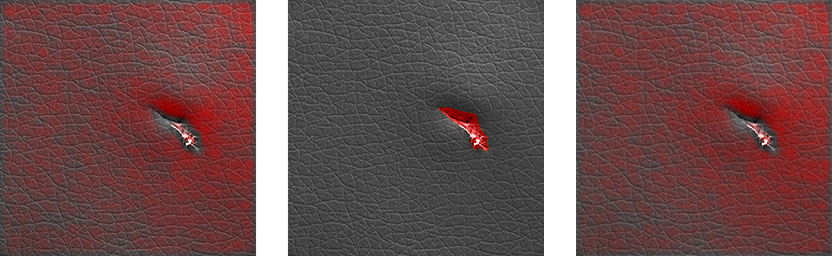
\includegraphics[width=\textwidth]{imgs/samples/leather_cut_anomap.jpg}
\caption{Example of an anomalous image from the leather category comparing MSA, the dataset mask and MLSA}
\label{fig:results:leather-anomap}
\end{figure}

\begin{figure}[ht!]
\centering

\includegraphics[width=\textwidth]{imgs/samples/leather_poke_recon.jpg}
\caption{Example of reconstructions from the leather category comparing MSA, the original and MLSA}
\label{fig:results:leather-recon}
\end{figure}

\begin{figure}[ht!]
\centering
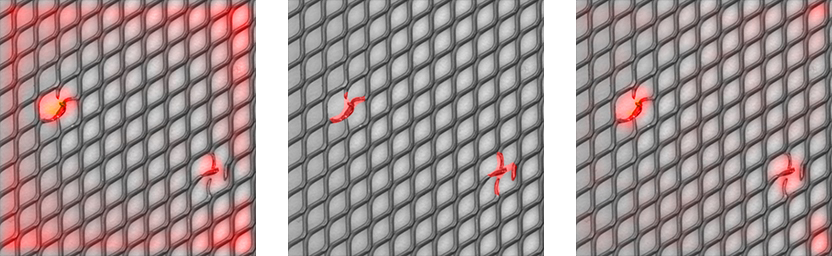
\includegraphics[width=\textwidth]{imgs/samples/grid_broken_anomap.jpg}
\caption{Example of an anomalous image from the grid category comparing MSA, the dataset mask and MLSA}
\label{fig:results:grid-anomap}
\end{figure}

It is interesting to see that the models do not perform the best for the majority of the images for detection and segmentation, but only for one of these tasks. Since the score for detection depends on the anomaly map that is used to calculate the score for segmentation we would expect the segmentation score to directly relate to the detection score.



\

Overall our numbers show that MLSA gives us better results, both for segmentation and detection on textured and object images. And for detection on texture images.

\iffalse
\begin{itemize}
\item Detection on textured is MLSA best, only the carpet and grid seem to actually really do much better
\item Segmentation on textured is MSA best, which is interesting since detection uses those same values. Which could mean that there are a lot of false-positives for the detection -> needs a graph example
\item Wood seems to do the best in all cases, need to check the images to see what is different with the other textures

\item Segmentation on objects: MLSA is best, detection we see 50/50
\item Especially for detection there are a few very low values: cable & pill
\item Image size of pill & screw is 320 & 512 which is the largest and is also where MSA wins
\item On average MLSA does seem to perform better, so depending on how much time it takes it to train it could be a good alternative
\end{itemize}
\fi

\begin{table}
\centering
\resizebox{\linewidth}{!}{%
\begin{tabular}{l|cc|cc|c} 
\toprule
Category        & \multicolumn{2}{l}{MSA}  & \multicolumn{2}{l}{MLSA} & Image size  \\ 
\midrule
                & Segmentation & Detection & Segmentation & Detection &             \\ 
\midrule
Carpet          & 90.44        & 77.09     & \textbf{91.52}        & \textbf{86.40}     & 512         \\
Grid            & 89.82        & 76.61     & \textbf{93.39}        & \textbf{89.97}     & 256         \\
Leather         &  49.99       & \textbf{86.85}     &     \textbf{56.23}    & 75.44     & 512         \\
Tile            & \textbf{79.31}        & 71.32     & 73.33        & \textbf{73.92}     & 512         \\
Wood            & \textbf{70.22}        & \textbf{77.54}     & 62.84        & 72.72     & 512         \\ 
\midrule
Texture average & \textbf{75.96} &	77.88 &	75.46 &	\textbf{79.69} &             \\ 
\midrule
Bottle          & 65.82        & \textbf{91.51}     & \textbf{68.65}        & 89.92     & 256         \\
Cable           & 88.04        & 38.17     & \textbf{90.07}        & \textbf{43.65}     & 256         \\
Capsule         & 81.66        & \textbf{72.32}     & \textbf{88.43}        & 66.33     & 320         \\
Hazelnut        & 67.94        & \textbf{55.89}     & \textbf{81.59}        & 53.82     & 256         \\
Metal nut       & 54.99        & 60.95     & \textbf{67.51}        & \textbf{78.49}     & 256         \\
Pill            & \textbf{88.60}        & 44.82     & 88.45        & \textbf{51.28}     & 320         \\
Screw           & \textbf{97.31}        & 55.69     & 97.23        & \textbf{65.32}     & 320         \\
Toothbrush      & 80.42        & 86.67     & \textbf{81.78}        & \textbf{87.22}     & 256         \\
Transistor      & 77.72        & \textbf{59.25}     & \textbf{79.95}        & 56.71     & 256         \\
Zipper          & \textbf{81.22}        & \textbf{79.07}     & 79.66        & 78.07     & 512         \\ 
\midrule
Object average  & 78.37        & 64.43     & \textbf{82.33}        & \textbf{67.08}     &             \\ 
\midrule
All average     & 80.02        & 66.46     & \textbf{81.32}        & \textbf{70.00}     &             \\
\bottomrule
\end{tabular}
}
\label{table:results:segdet}
\caption{Results in ROC AUC \% for segmentation and detection}
\end{table}




\section{Efficiency}
\label{sec:results:efficiency}

\textit{How does the number of epochs required to get the best result compare across images with different textures and objects?}\

The number of epochs required depends on the type of image. Image that have more complex structures require more epochs. We see this especially in the texture category and for the cable, screw and transistor images. Another factor affecting the number of epochs is the amount of colours used. This is shown by the pill and zipper images that both require a very low number of epochs and primarily consist of black, white and grey colours. We give some samples of the image categories in figure \ref{fig:results:detail-samples}.

\begin{figure}[ht!]
\centering
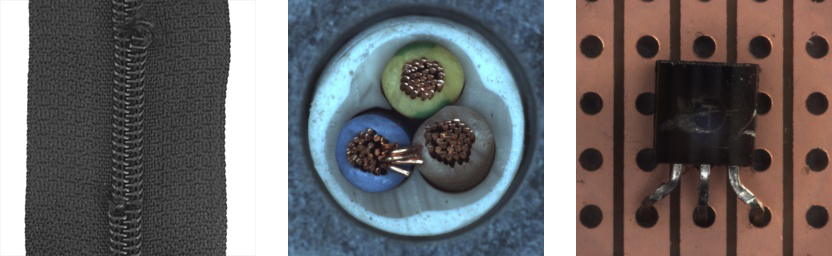
\includegraphics[width=\textwidth]{imgs/samples/image-detail-sample.jpg}
\caption{Examples of the zipper, cable and transistor image types}
\label{fig:results:detail-samples}
\end{figure}

\textit{How does the training time compare between the full and linear attention models across images with different textures and objects?}\

We see that the time per epoch is lower for MSA in all categories except for the pill and transistor images. With this information we would expect the MSA models to also finish training faster. The opposite is true however, since the number of epochs required for the best result is lower in eleven of the fifteen cases the total training time is lower for MLSA.

\iffalse
\begin{itemize}
    \item Time per epoch is lower for MSA in all categories except for pill and transistor
    \item Less epochs to get the best result in the case of MSA: 2, 11 for MLSA, 3 the same
    \item The above would mean that given the number of epochs is lower, the total time is also lower
    \item given that in the previous section it is also better in the task the linear model is slightly better
    \item Training time does highly depend on the category, but there is no clear difference except for the object images with a solid background seem to require less training time.
    \item The pill and zipper images that are technically black/white do require the lowest number of epochs
\end{itemize}
\fi

\begin{table}
\centering
\resizebox{\linewidth}{!}{%
\begin{tabular}{l|ccc|ccc} 
\toprule
Category   & \multicolumn{3}{l}{MSA}                 & \multicolumn{3}{l}{MLSA}                 \\ 
\midrule
~          & Best epoch & Time/Epoch & Training time & Best epoch & Time/Epoch & Training time  \\ 
\midrule
Carpet     & 77         & 0:58:05    & 220:42:00     & 138        & 1:07:17    & 265:47:00      \\
Grid       & 140        & 0:26:48    & 130:00:00     & 53         & 0:33:34    & 114:06:00      \\
Leather    & 142        & 0:43:50    & 214:03:00     & 142        & 0:43:33    & 213:24:00      \\
Tile       & 353        & 0:36:40    & 308:01:00     & 555        & 0:39:38    & 466:23:00      \\
Wood       & 149        & 0:53:56    & 270:33:00     & 124        & 0:56:16    & 258:49:00      \\
\midrule
Bottle     & 37         & 0:24:11    & 75:47:00      & 11         & 0:24:33    & 66:16:00       \\
Cable      & 250        & 0:39:59    & 267:55:00     & 211        & 0:48:07    & 267:05:00      \\
Capsule    & 27         & 0:41:38    & 123:30:00     & 14         & 0:41:45    & 114:50:00      \\
Hazelnut   & 83         & 1:22:12    & 321:56:00     & 19         & 1:25:10    & 242:43:00      \\
Metal nut  & 148        & 0:25:31    & 127:10:00     & 43         & 0:28:22    & 91:42:00       \\
Pill       & 5          & 0:48:57    & 128:06:00     & 4          & 0:46:54    & 121:57:00      \\
Screw      & 245        & 0:40:27    & 267:01:00     & 211        & 0:40:37    & 245:04:00      \\
Toothbrush & 58         & 0:12:19    & 42:55:00      & 58         & 0:12:10    & 42:24:00       \\
Transistor & 271        & 0:46:40    & 328:13:00     & 196        & 0:44:59    & 260:57:00      \\
Zipper     & 5          & 0:25:59    & 67:34:00      & 5          & 0:34:52    & 90:39:00       \\
\bottomrule
\end{tabular}
}
\label{table:results:times}
\caption{Best epochs and time taken to finish training}
\end{table}

\section{Compared to previous work}

\textit{How do our results compare to previous work?}

When we compare our results to the values from the original InTra model by Pirnay et al. \cite{pirnay_inpainting_2021} in table \ref{table:results:pirnay} we see that the performance of our models is worse than the original implementation. The only result that is better is the segmentation for the carpet image type. This was to be expected, since we have omitted some parts of the original InTra model that improved their results.

\begin{table}
\centering
\begin{tabular}{l|cc} 
\toprule
Category        & \multicolumn{2}{l}{InTra}    \\ 
\midrule
                & Segmentation & Detection    \\ 
\midrule
Carpet          & 88.2         & 98           \\
Grid            & 98.8         & 100          \\
Leather         & 99.5         & 100          \\
Tile            & 94.4         & 98           \\
Wood            & 88.7         & 97          \\ 
\midrule
Texture average & 96.1         & 98           \\ 
\midrule
Bottle          & 97.1         & 100          \\
Cable           & 91.0         & 70           \\
Capsule         & 97.7         & 86           \\
Hazelnut        & 98.3         & 95         \\
Metal nut       & 93.3         & 96          \\
Pill            & 98.3         & 90          \\
Screw           & 99.5         & 95          \\
Toothbrush      & 98.9         & 100         \\
Transistor      & 96.1         & 95          \\
Zipper          & 99.2         & 99          \\ 
\midrule
Object average  & 96.9         & 93          \\ 
\midrule
All average     & 96.6         & 95          \\
\bottomrule
\end{tabular}
\label{table:results:pirnay}
\caption{Results from \cite{pirnay_inpainting_2021}}
\end{table}

\iffalse
\begin{itemize}
    \item Results are much worse
    \item Different attention function
    \item No connections between layers
    \item No augmentations
\end{itemize}
\fi
\chapter{Conclusions}\label{ch:conclusions}

In this thesis we have shown that we can use visual transformers with a linear attention function to tackle an anomaly detection problem using inpainting. Our primary goal was to answer the main research question we asked in the introduction: \textsl{What is the effect on the performance and efficiency of using linear transformers in an inpainting context for anomaly detection when compared to regular transformers?}

To answer this question we have successfully implemented two types of models for inpainting: one using regular transformers and one using linear transformers. To evaluate our models they have been trained on the MVTec AD dataset and the results of the inpainting task were used to perform anomaly detection. This required us to calculate anomaly maps using the MSGMS metric that we were able to compare with the masks provided by the dataset.

The results show that linear transformers are able to outperform the regular transformers in the tasks of segmentation and detection. They require less epochs to be able to converge, however in contrast to what we would have expected the time per epoch is longer for these models.

This should answer our primary research question. However, we think that our results should be viewed with caution. It is possible that parts of our implementation affect the resource usage negatively and therefore the time required to train our models.

For future work our models could be revisited to find the resource usage of the different parts like the data loader and metrics functions. An in-depth analysis of the resource usage of these parts could give a better insight to understand our results.

Another change could be adding augmentations to the data loader to see if this would improve the results. As well as hyperparameter optimisation. It might be possible that the different visual transformers can reach better results with other parameters than those that we re-used from other papers. As well as changing the evaluation and the loss function to find better options that would be better suited for the reconstruction task.

Different approaches using linear transformers could also be explored. For example by using linear transformers for feature extraction in a similar approach like the one introduced in \cite{yu_fastflow_2021}.

Apart from using the linear transformers in another context it is also an option to use fastformers \cite{wu_fastformer_2021} or linformers \cite{wang_linformer_2020} in this context of anomaly detection. This would allow us to evaluate the performance of multiple transformer based approaches to see the effects when compared to regular transformers.

\bibliographystyle{acm}
\bibliography{references}

\appendix
\chapter{Dataset details}\label{ch:data}

An appendix, if you need one.

\newpage
\listoftodos[Notes]

\end{document}